\ifdefined\isdraft
   \documentclass[25pt, landscape, draft]{foils}
\else
   \documentclass[25pt, landscape, final]{foils}
\fi

\usepackage{geometry}
\usepackage{graphicx}
\usepackage[usenames,dvipsnames,svgnames]{xcolor}
\usepackage{amsmath,amssymb,amsfonts} % Typical maths resource packages
\usepackage{comment}
\usepackage[colorlinks=false,bookmarks=false,pageanchor=true]{hyperref}
\usepackage{authblk}
\usepackage{pstricks}
\usepackage{pst-node}

% Requires \documentclass{foils} in the preamble
\newcommand{\myfoilhead}[2]{\foilhead[#1]{\textcolor{blueDark}{\boldmath #2}}}

% Basic commonly used commands
\renewcommand\labelitemi{\textcolor{redDark}{$\bullet$}}
\renewcommand\labelitemii{\textcolor{greenDark}{$\bullet$}}
\renewcommand\labelitemiii{\textcolor{blueDark}{$\bullet$}}

\newcommand\arabicitemii{\textcolor{greenDark}{\textbf{\arabic{listcounter}.}}}

% Requires color package
% \usepackage{color}

\definecolor{redDark}{rgb}{0.8,0,0}
\definecolor{blueDark}{rgb}{0,0,0.5}
\definecolor{blueLight}{rgb}{0.5, 0.4, 1.0}
\definecolor{blue1}{rgb}{0.8, 0.8, 1.0}
\definecolor{greenDark}{rgb}{0, .5, 0}
\definecolor{greenDark2}{rgb}{0, .4, 0}
\definecolor{greenLight}{rgb}{.8, 1.0, .8}
\definecolor{yellowDark}{rgb}{.6, .6, 0}
\definecolor{black}{rgb}{0, 0, 0}
\definecolor{yellow}{rgb}{1.0, 1.0, 0.0}
\definecolor{bgColor}{rgb}{1,1,1}
\definecolor{pink}{rgb}{1.0,0.9,0.9}
\definecolor{greyLight}{rgb}{0.8,0.8,0.8}
\definecolor{greyDark}{rgb}{0.4,0.4,0.4}


\AtBeginDocument{\color{blueDark}}

% The chosen paper size has aspect ratio of 1.6. It is a compramize between the
% varios standard paper sizes and the typical screen/projector aspect ratio of
% 16:9
\geometry{paperwidth=320mm, paperheight=200mm, includeall=true,
          centering=true, nomarginpar, headsep=0mm, headheight=0mm,
          tmargin=1mm, bmargin=1mm, lmargin=1mm, rmargin=1mm}

\hypersetup {
   pdfauthor={Dmitri Smirnov <d.s@plexoos.com>}
}


\MyLogo{}
\leftheader{}
\rightheader{\footnotesize \thepage}
\rightfooter{}
\Restriction{}

\setlength{\unitlength}{0.02\textwidth}
\psset{unit=\unitlength}
\psset{framearc=.1,fillcolor=blueDark!10,linecolor=blueDark,linewidth=0.1,fillstyle=solid,arrowscale=3}


\title{\vspace{20mm} \Large Vertex Reconstruction\\[3mm] with STAR muDST Data Format}

\author{\quad\\[3mm]
Dmitri~Smirnov}

\affil{BNL}

\date{\small January 12, 2017}


\newcommand{\StMuTrack}{\texttt{StMuTrack}}
\newcommand{\StTrack}{\texttt{StTrack}}



%===============================================================================
\begin{document}

\maketitle
\addtocounter{page}{1}

\small


\begin{comment}

%===============================================================================
\myfoilhead{-30mm}{Current State}
%{{{

\noindent
\begin{pspicture}(0,0)(\textwidth,\textheight)



\rput(0.50\textwidth,0.45\textheight) {%
\begin{minipage}{0.90\textwidth}

\raggedright

\begin{list}{\labelitemi}{\setlength{\itemsep}{0mm}
                          \setlength{\topsep}{0mm}}

   \item Vertex reconstruction at STAR is integral part of full event reconstruction

   \begin{list}{\labelitemii}{\setlength{\itemsep}{3mm}
                              \setlength{\topsep}{0mm}}

      \item Raw data files (.daq)

   \end{list}

   \item Propose to run vertex finders over muDst files


   \fbox{%
   \begin{minipage}{0.44\textwidth}

   Pros

   \begin{list}{\labelitemii}{\setlength{\itemsep}{3mm}
                              \setlength{\topsep}{0mm}}

      \item No need to create track DCAs

   \end{list}

   \end{minipage} }
   %
   \fbox{%
   \begin{minipage}{0.44\textwidth}

   Cons

   \begin{list}{\labelitemii}{\setlength{\itemsep}{3mm}
                              \setlength{\topsep}{0mm}}

      \item

   \end{list}

   \end{minipage} }

\end{list}

\end{minipage}
}



%\psgrid[gridlabels=0.7,subgriddiv=0, griddots=3](1,-1)(0,-3)(\textwidth,\textheight)

\end{pspicture}
%}}}

\end{comment}



%===============================================================================
\myfoilhead{-30mm}{Some Implementation Details}
%{{{

\noindent
\begin{pspicture}(0,0)(\textwidth,\textheight)



\rput(0.50\textwidth,0.45\textheight) {%
\begin{minipage}{0.90\textwidth}

\raggedright

\begin{list}{\labelitemi}{\setlength{\itemsep}{0mm}
                          \setlength{\topsep}{0mm}}

   \item Currently focus on PPV

   \item In muDst VF track selection loose $\lesssim 10\%$ of tracks (if start from the same set)

   \item Vertex daughters assigned at final stage

   \begin{list}{\labelitemii}{\setlength{\itemsep}{3mm}
                              \setlength{\topsep}{0mm}}

		\item If track was used in seeding OR $ d/(\sigma_\text{DCA} + \sigma_\text{vertex}) < 2$ (fully correlated
				$\sigma_\text{DCA}$ and $\sigma_\text{vertex}$)

   \end{list}

\end{list}

\end{minipage}
}



%\psgrid[gridlabels=0.7,subgriddiv=0, griddots=3](1,-1)(0,-3)(\textwidth,\textheight)

\end{pspicture}
%}}}



%===============================================================================
\myfoilhead{-30mm}{muDst Reco vs. Std Reco}
%{{{

\noindent
\begin{pspicture}(0,0)(\textwidth,\textheight)

\rput[rt](0.5\textwidth,22){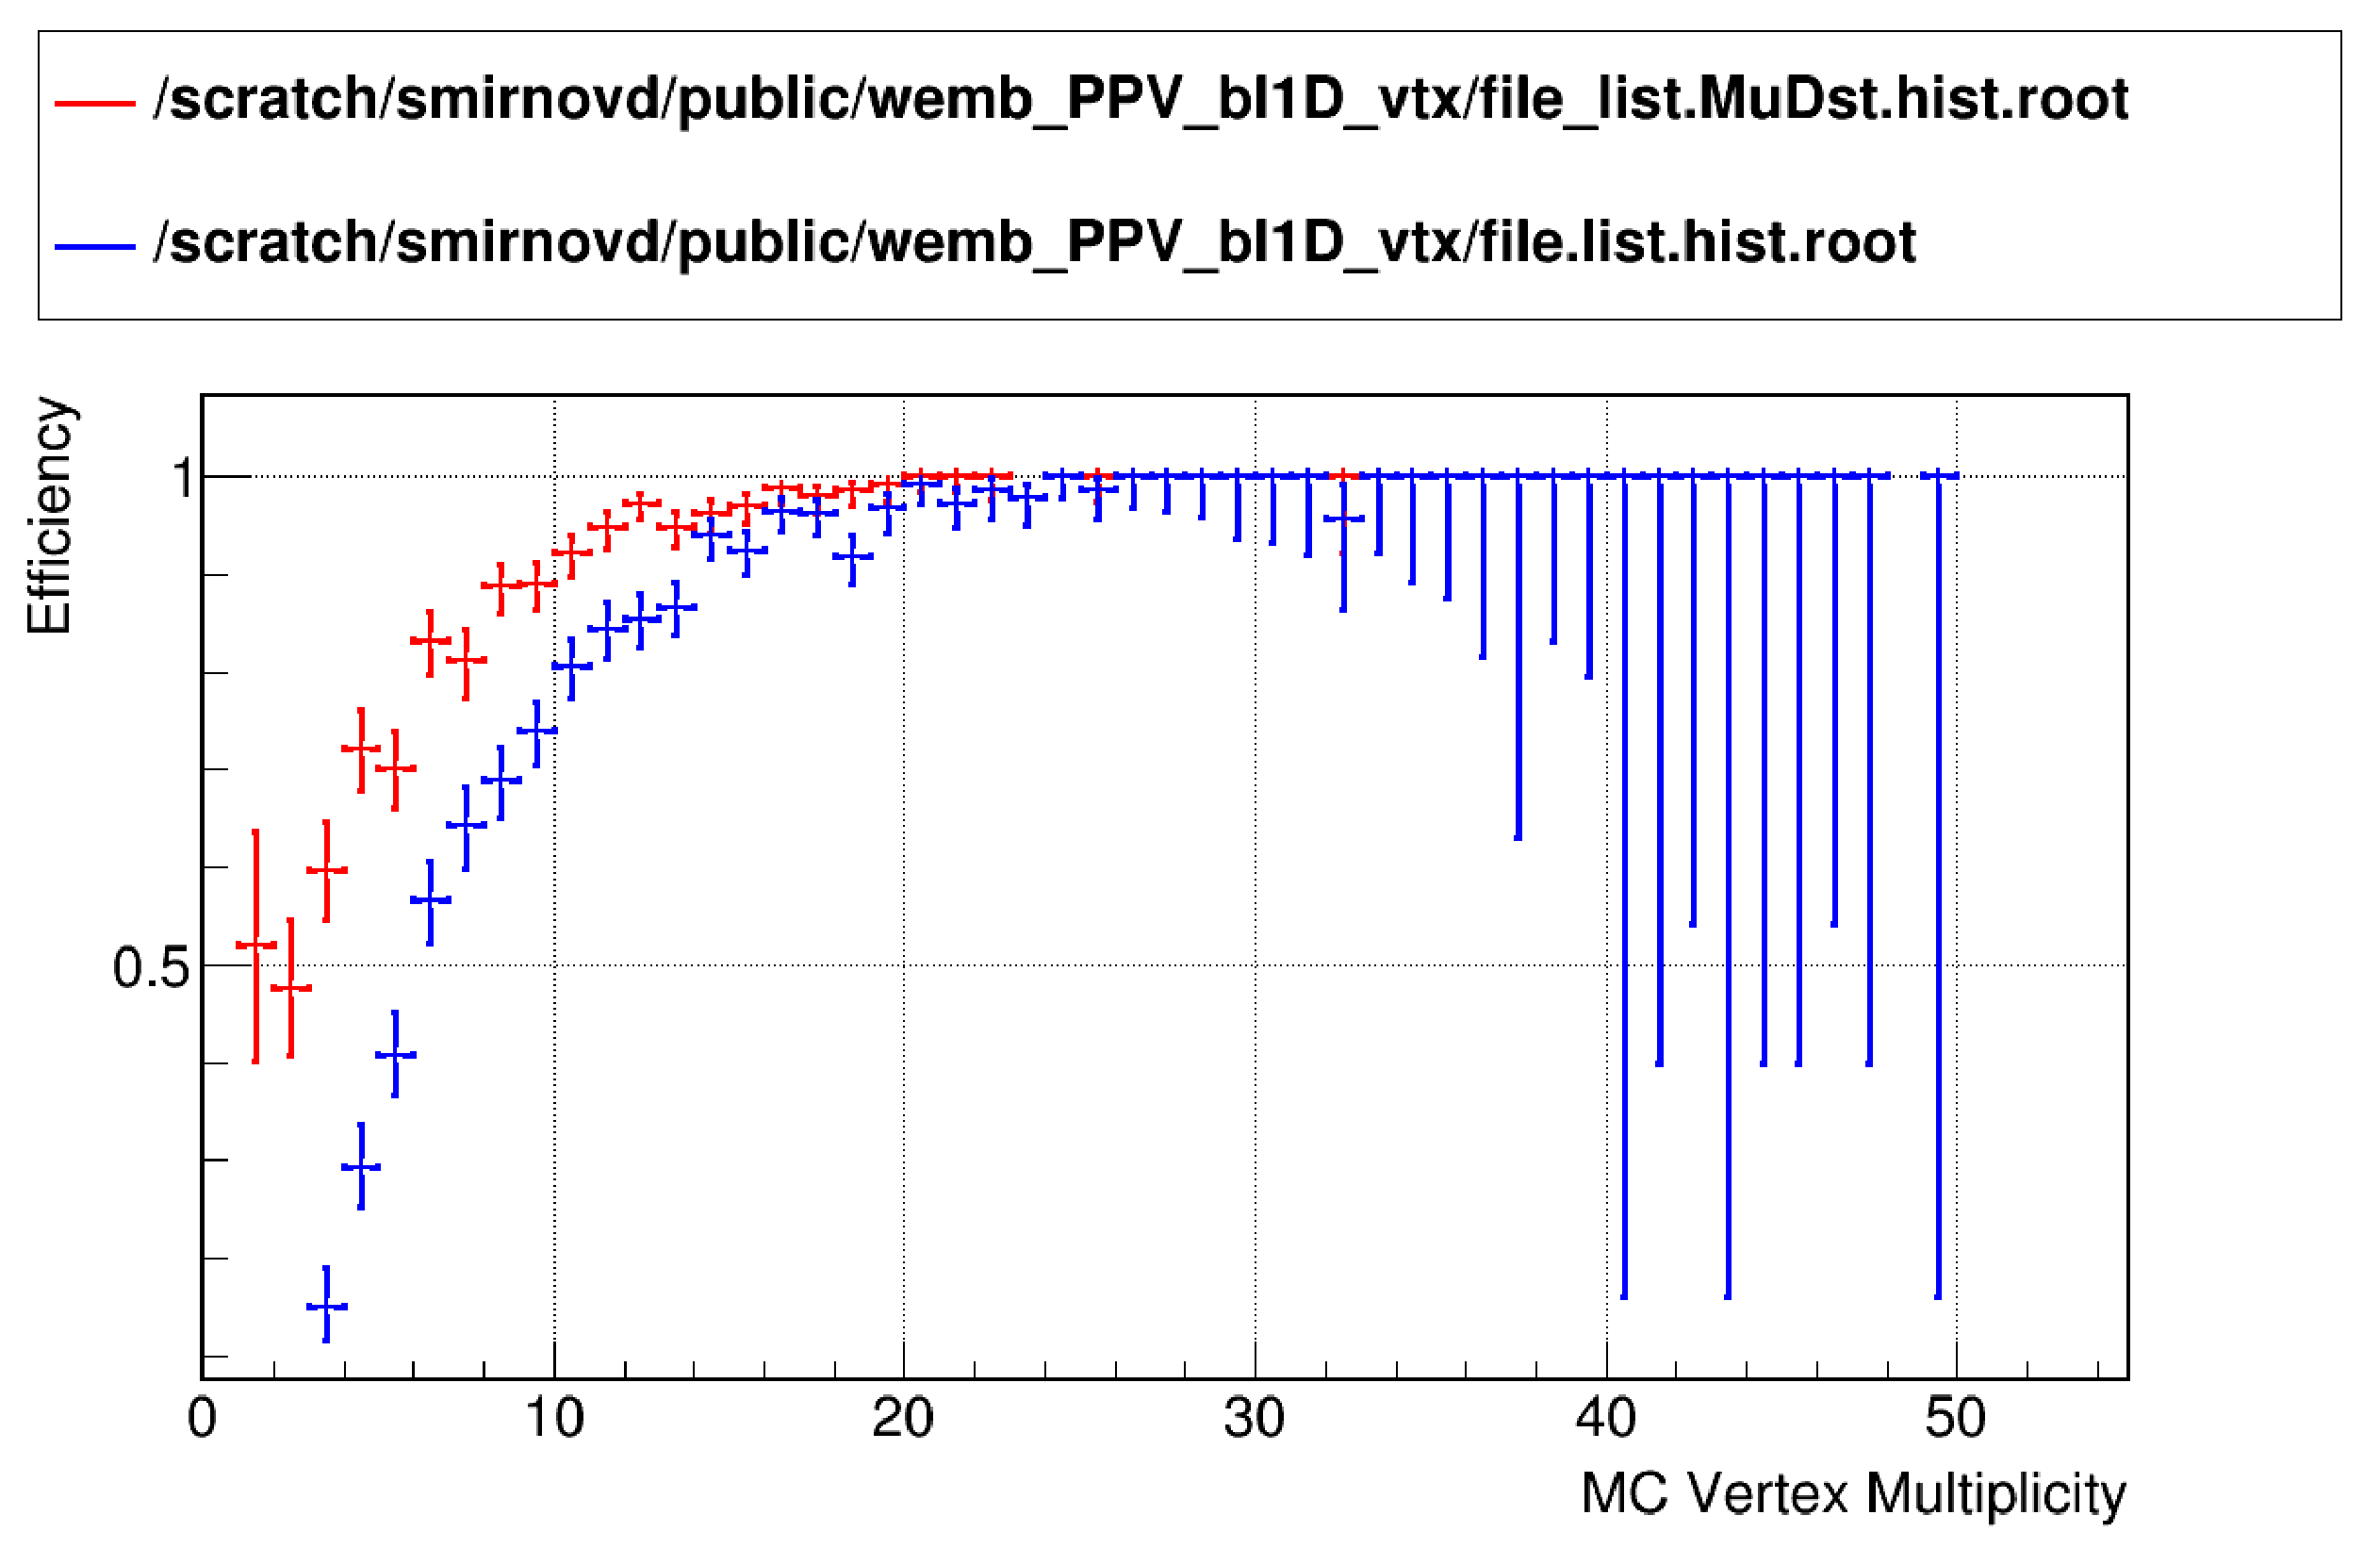
\includegraphics[height=0.5\textheight]{graphics/wemb_PPV_bl1D_muDst_vs_std_reco/event/McRecMulAny_eff}}
\rput[lt](0.5\textwidth,22){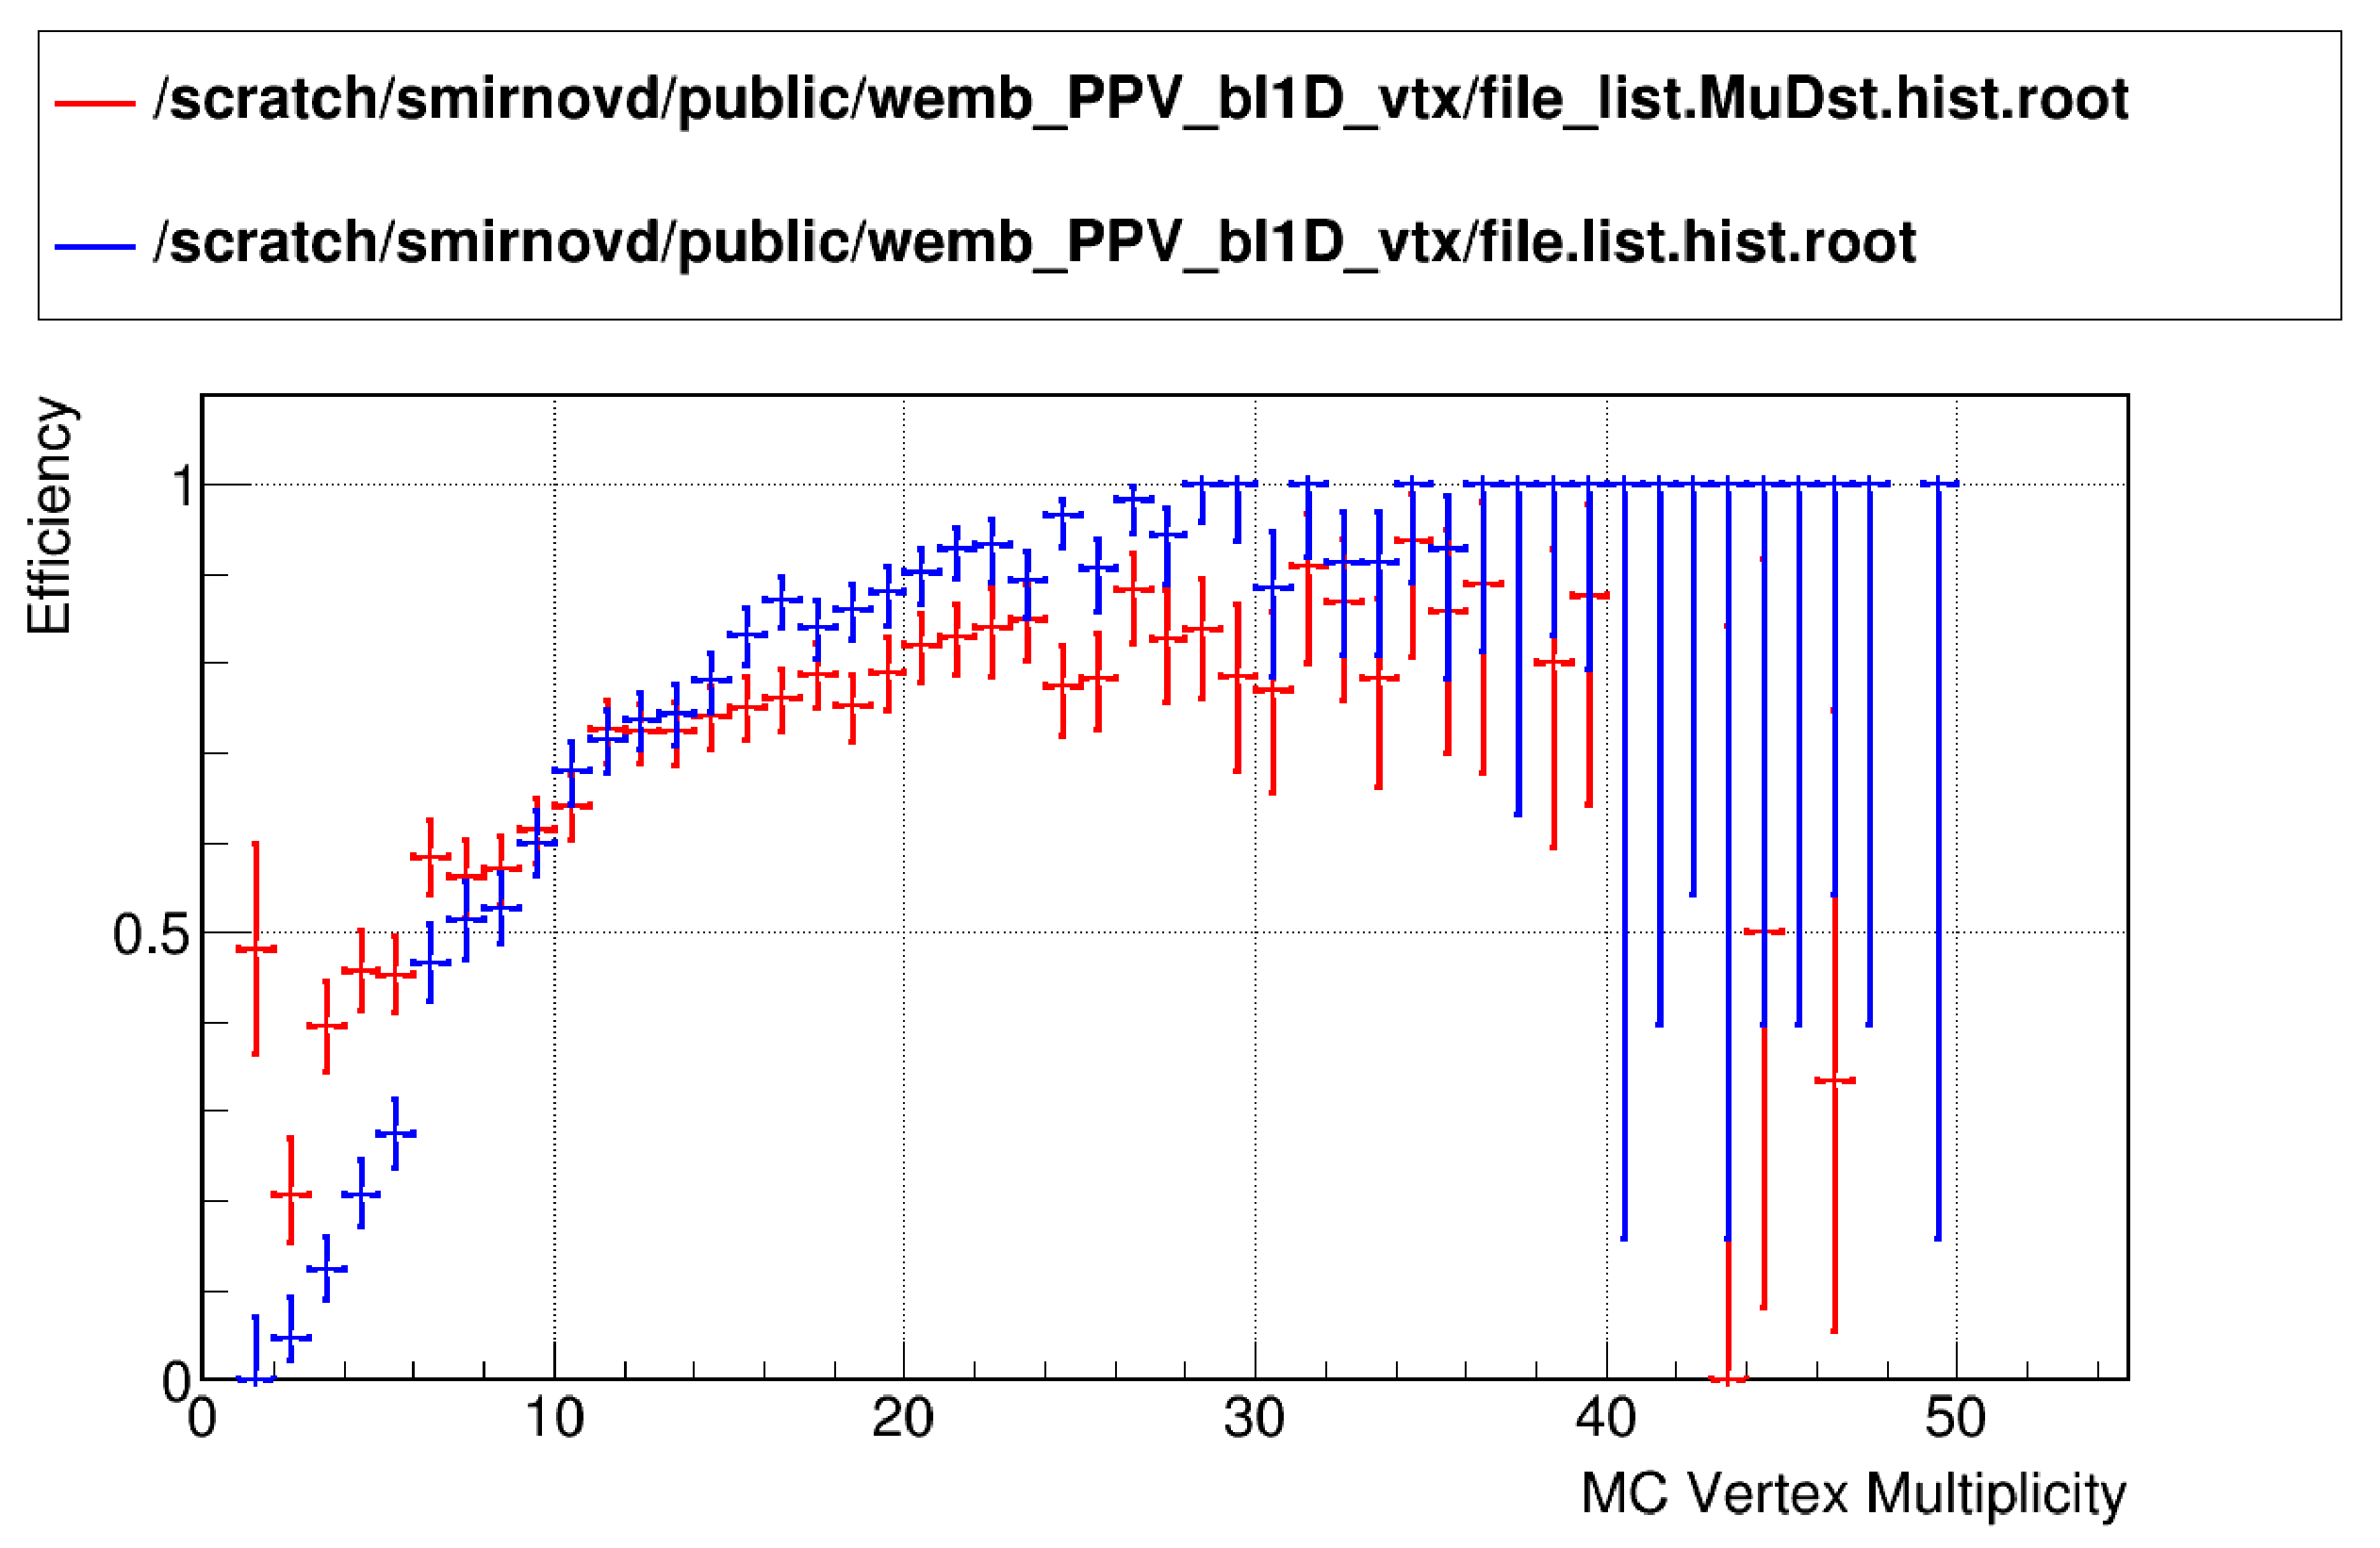
\includegraphics[height=0.5\textheight]{graphics/wemb_PPV_bl1D_muDst_vs_std_reco/event/McRecMulGood_eff}}


\rput(0.5\textwidth, 2) {%
\begin{minipage}{0.90\textwidth}

\raggedright

\begin{list}{\labelitemi}{\setlength{\itemsep}{0mm}
                          \setlength{\topsep}{0mm}}

   \item Case of PPV with 1D beamline fit
   \item 3D and no beamline cases look similar

\end{list}

\end{minipage}
}



%\psgrid[gridlabels=0.7,subgriddiv=0, griddots=3](1,-1)(0,-3)(\textwidth,\textheight)

\end{pspicture}
%}}}



%===============================================================================
\myfoilhead{-30mm}{Vertex Eff. With vs Without Cut on \StTrack-s}
%{{{

\noindent
\begin{pspicture}(0,0)(\textwidth,\textheight)

\rput[rt](0.5\textwidth,22){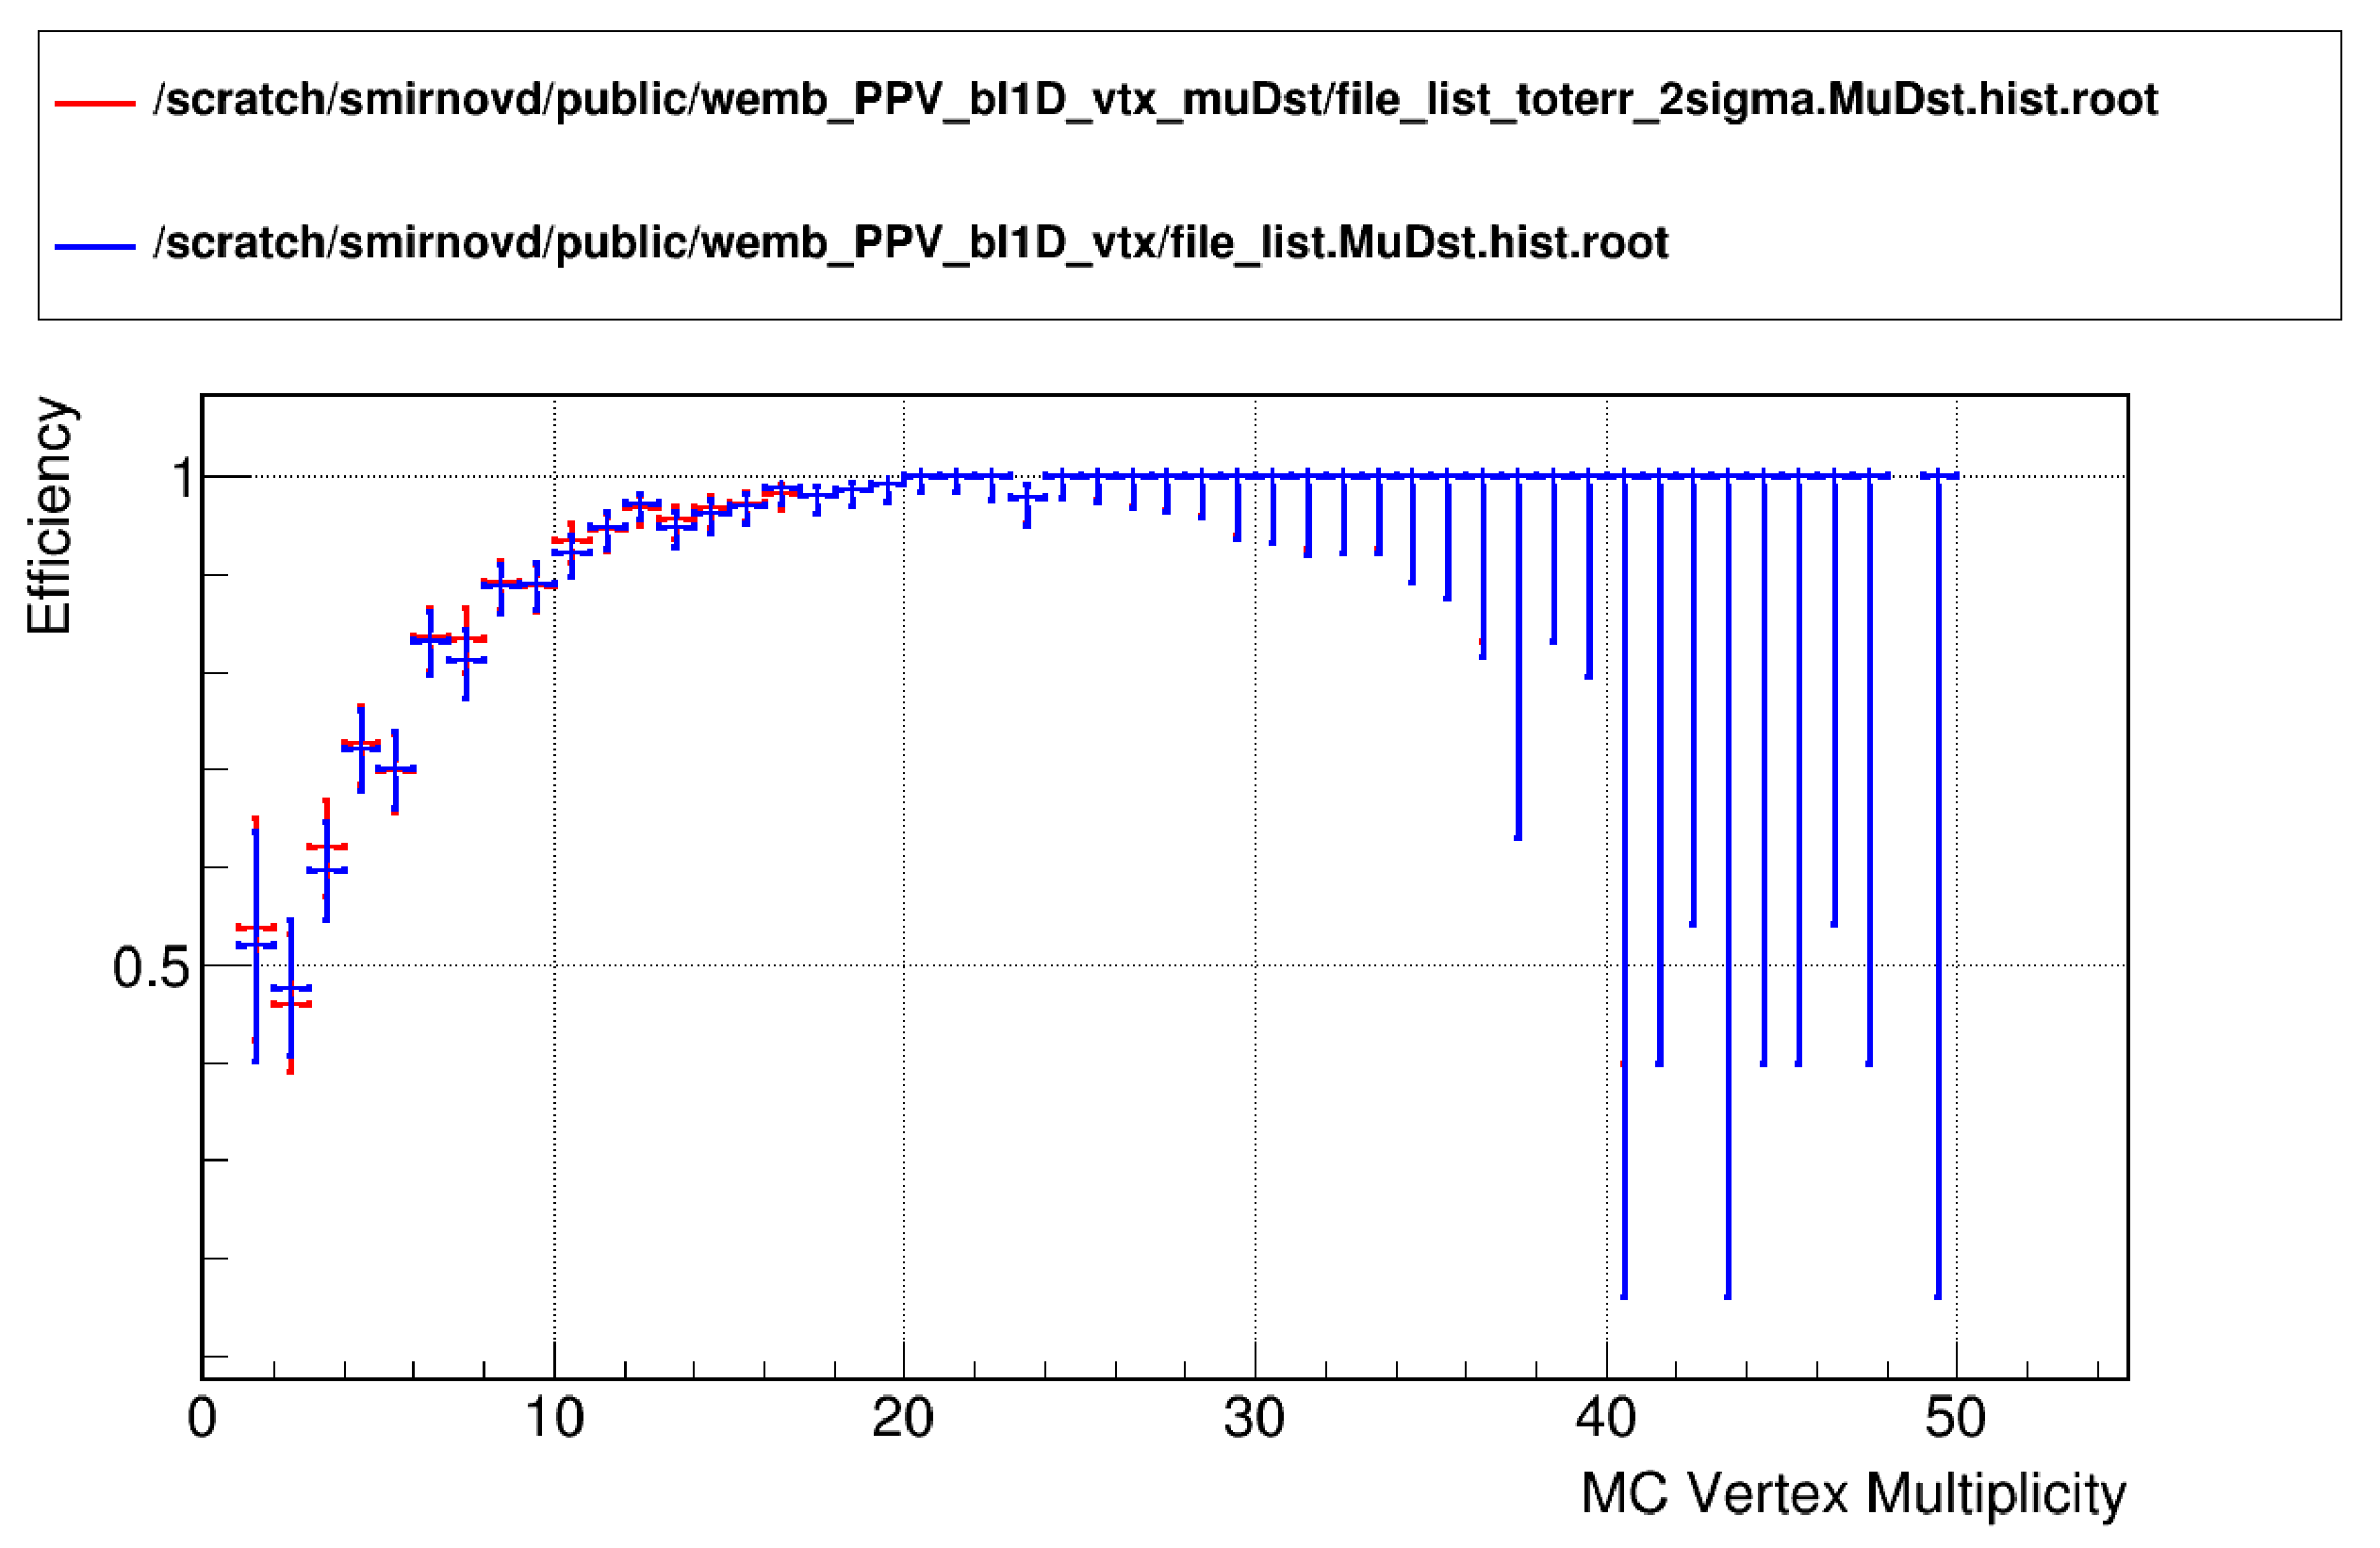
\includegraphics[height=0.5\textheight]{graphics/wemb_PPV_bl1D_muDst_reco_cut_nocut/event/McRecMulAny_eff}}
\rput[lt](0.5\textwidth,22){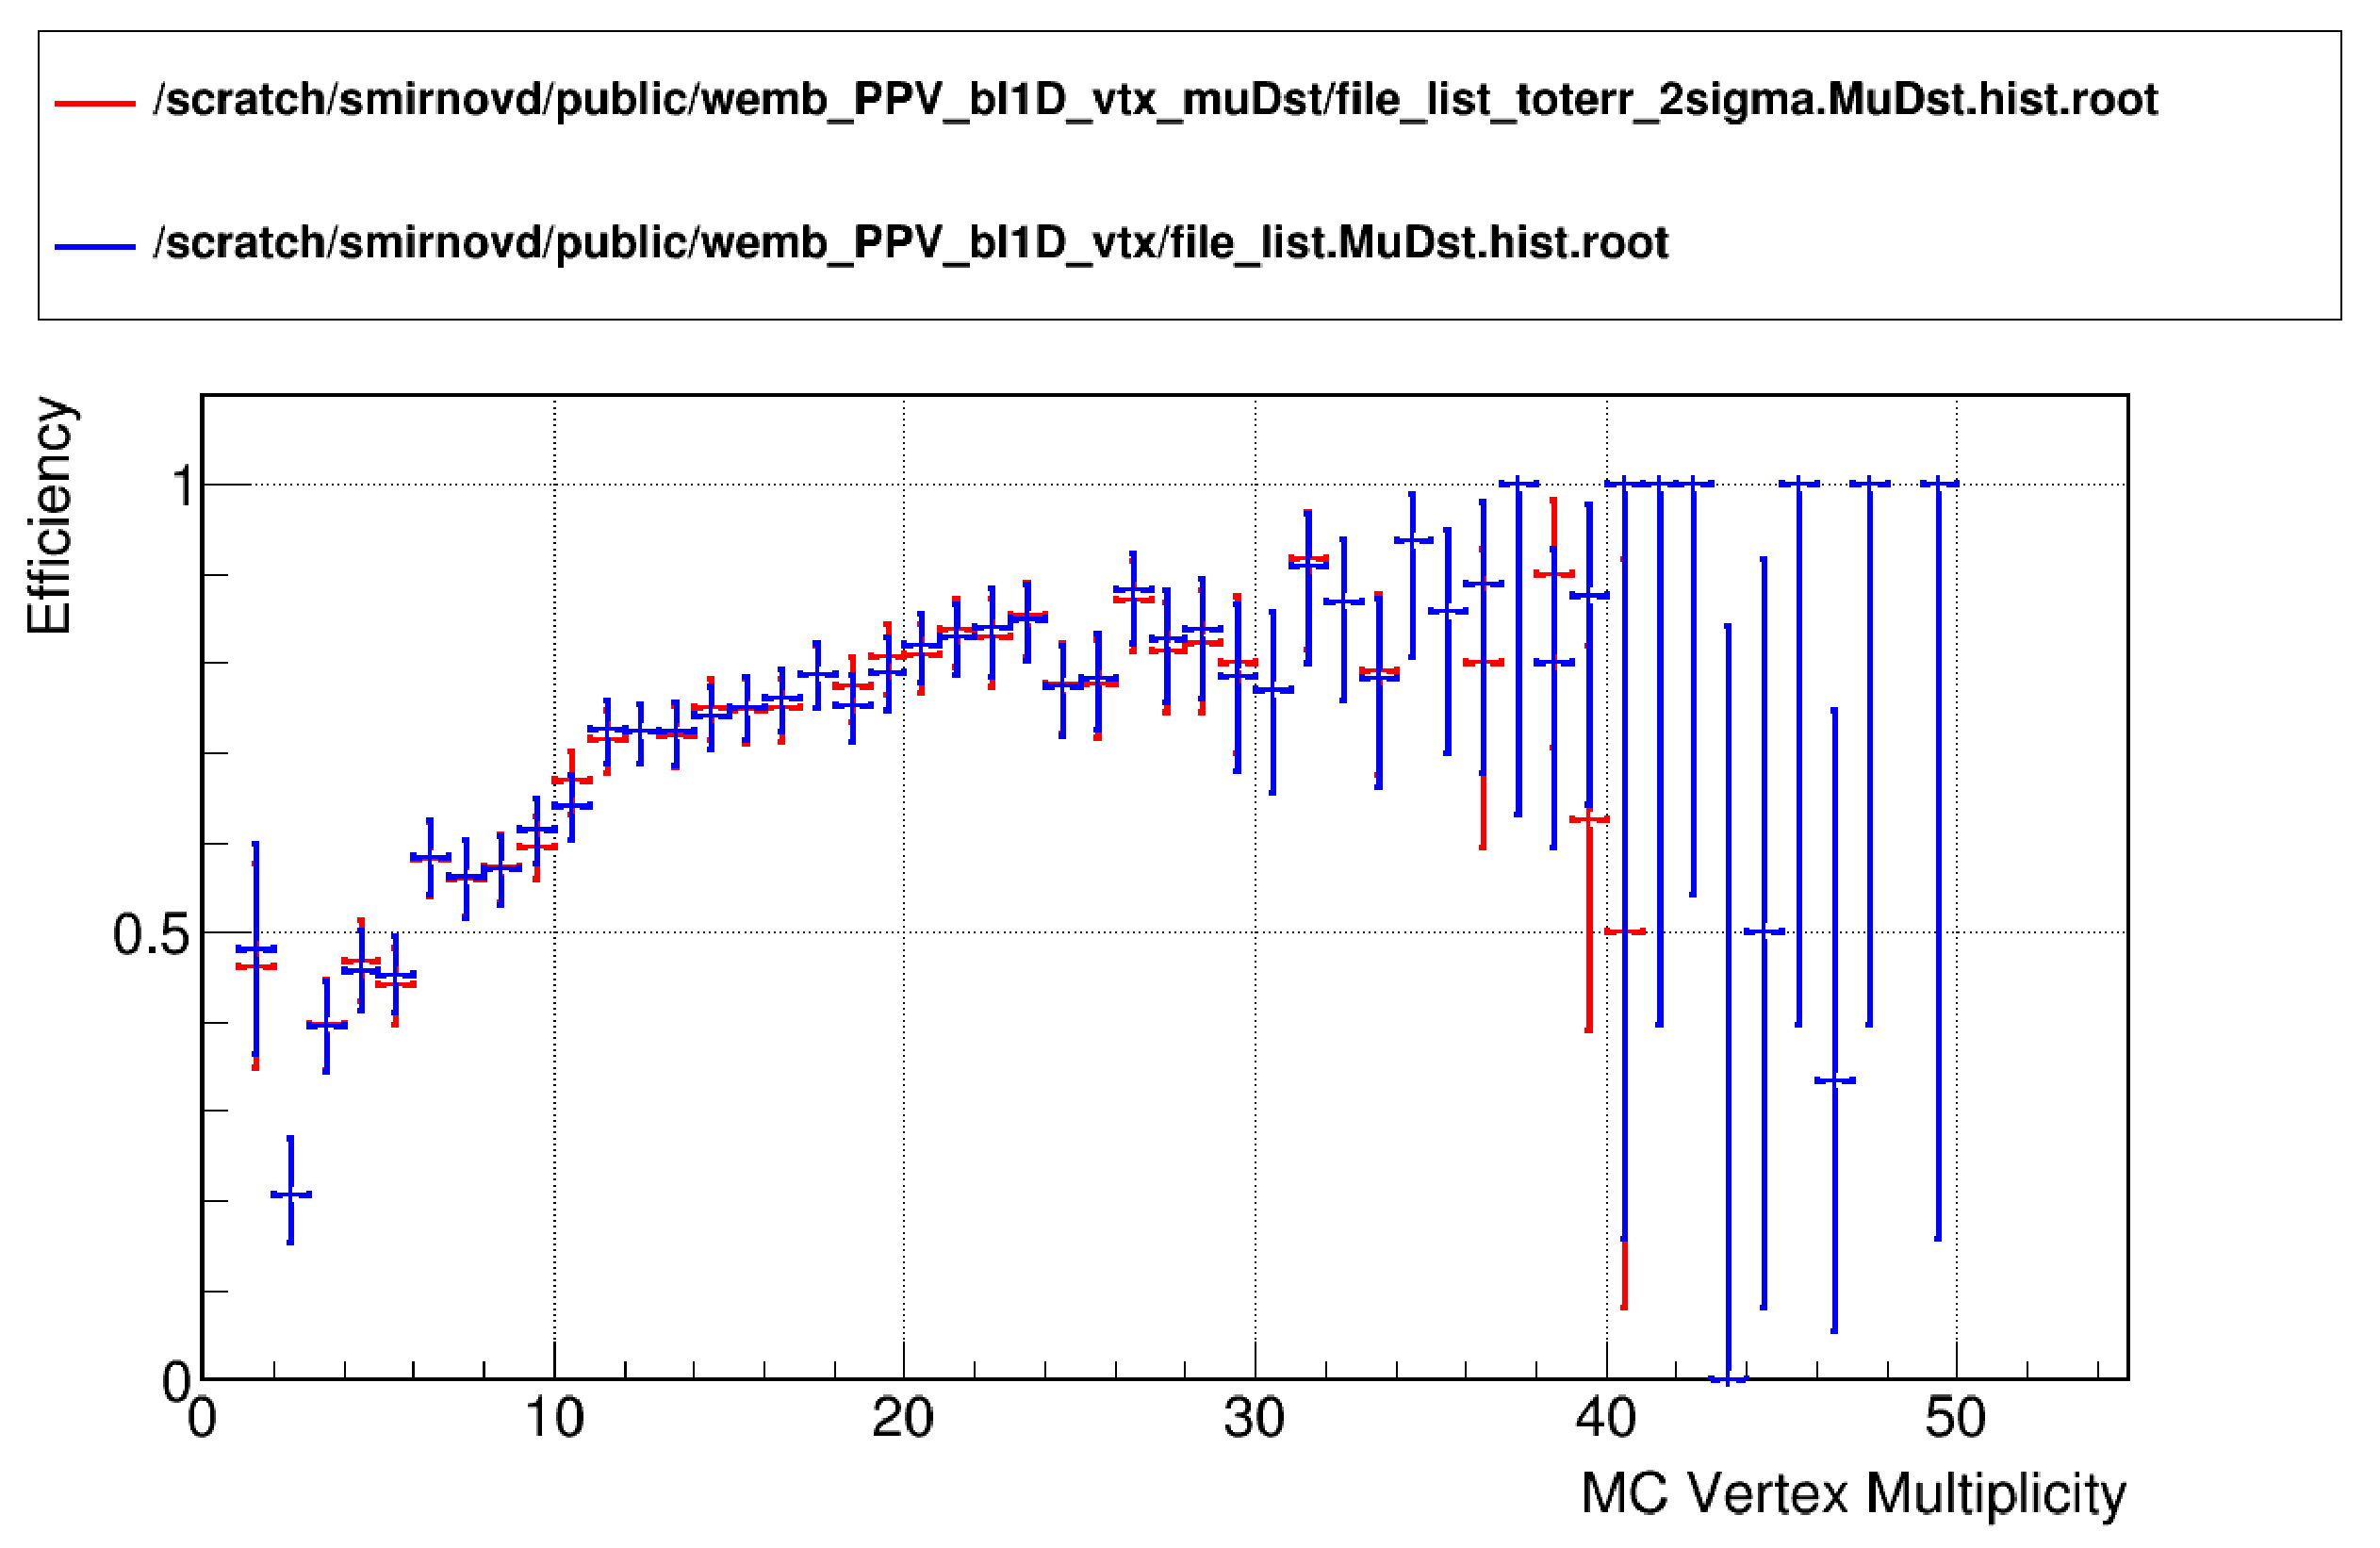
\includegraphics[height=0.5\textheight]{graphics/wemb_PPV_bl1D_muDst_reco_cut_nocut/event/McRecMulGood_eff}}


\rput(0.5\textwidth, 2) {%
\begin{minipage}{0.90\textwidth}

\raggedright

\begin{list}{\labelitemi}{\setlength{\itemsep}{0mm}
                          \setlength{\topsep}{0mm}}

   \item Efficiency does not change significantly when all \StTrack-s converted to \StMuTrack-s

\end{list}

\end{minipage}
}



%\psgrid[gridlabels=0.7,subgriddiv=0, griddots=3](1,-1)(0,-3)(\textwidth,\textheight)

\end{pspicture}
%}}}



%===============================================================================
\myfoilhead{-30mm}{Need to understand \ldots}
%{{{

\noindent
\begin{pspicture}(0,0)(\textwidth,\textheight)

\rput[rt](0.5\textwidth,25){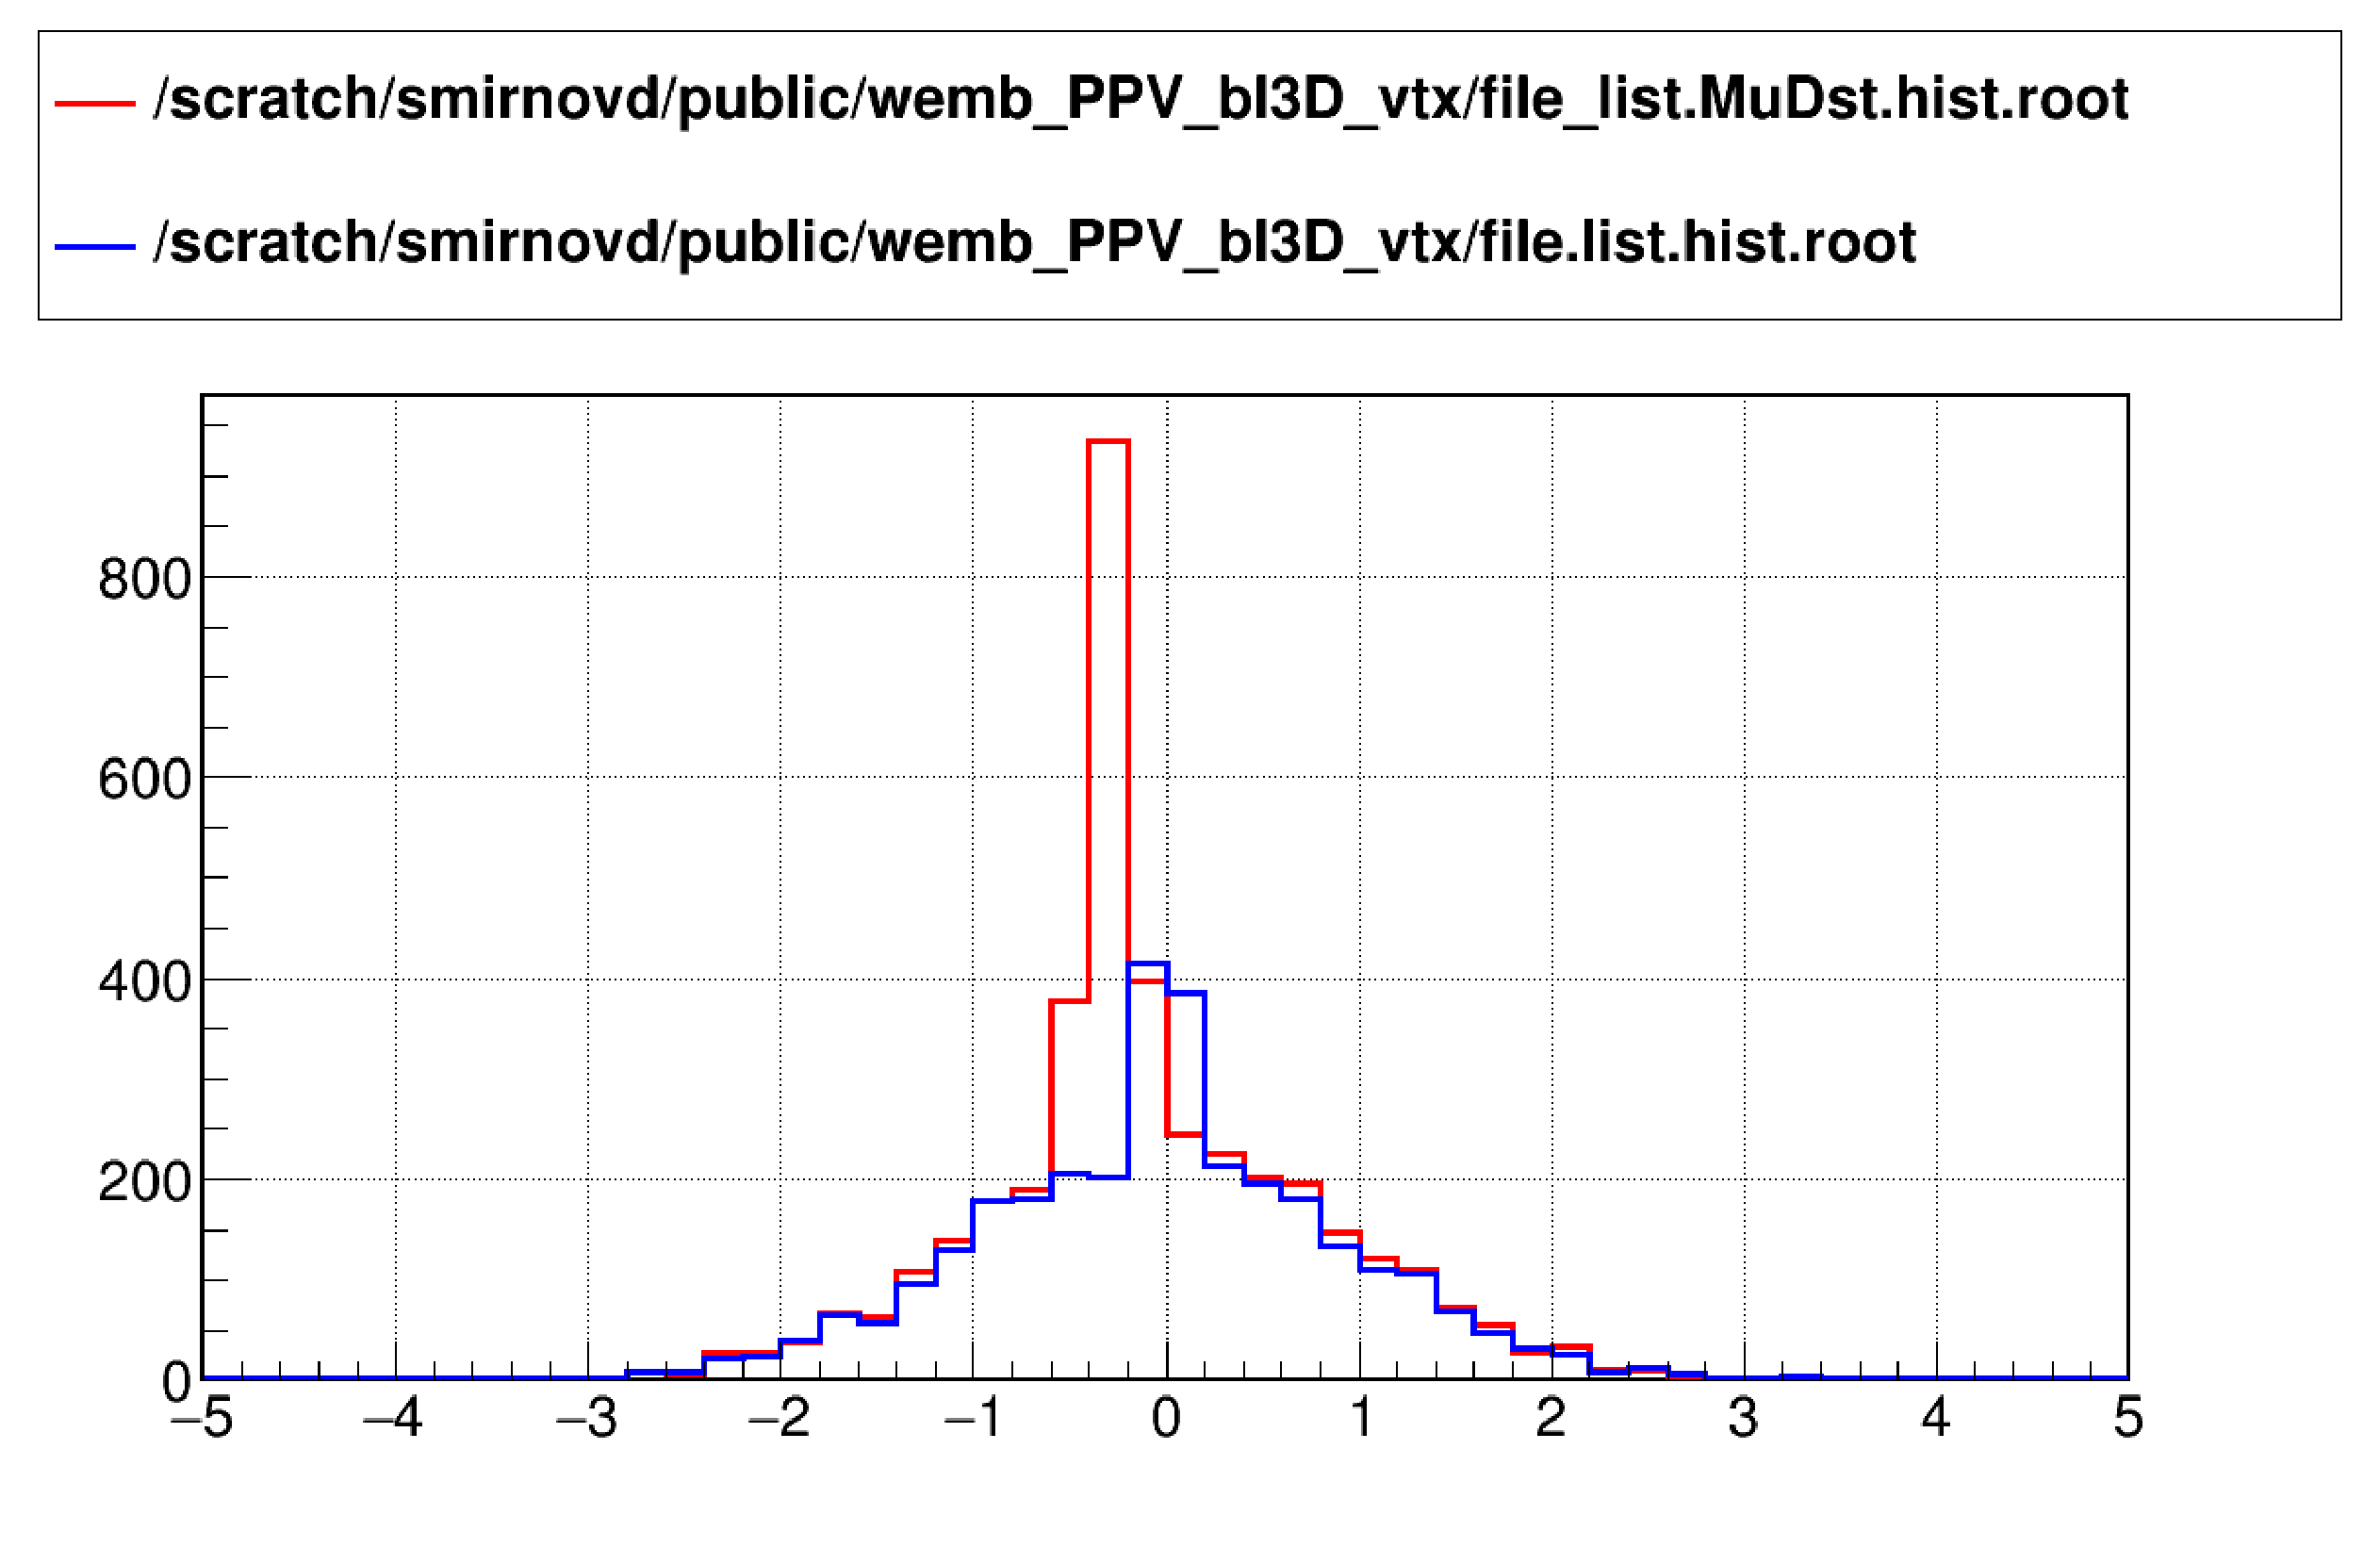
\includegraphics[height=0.5\textheight]{graphics/wemb_PPV_bl3D_muDst_vs_std_reco/vertex/hVertexPullX}}
\rput[lt](0.5\textwidth,25){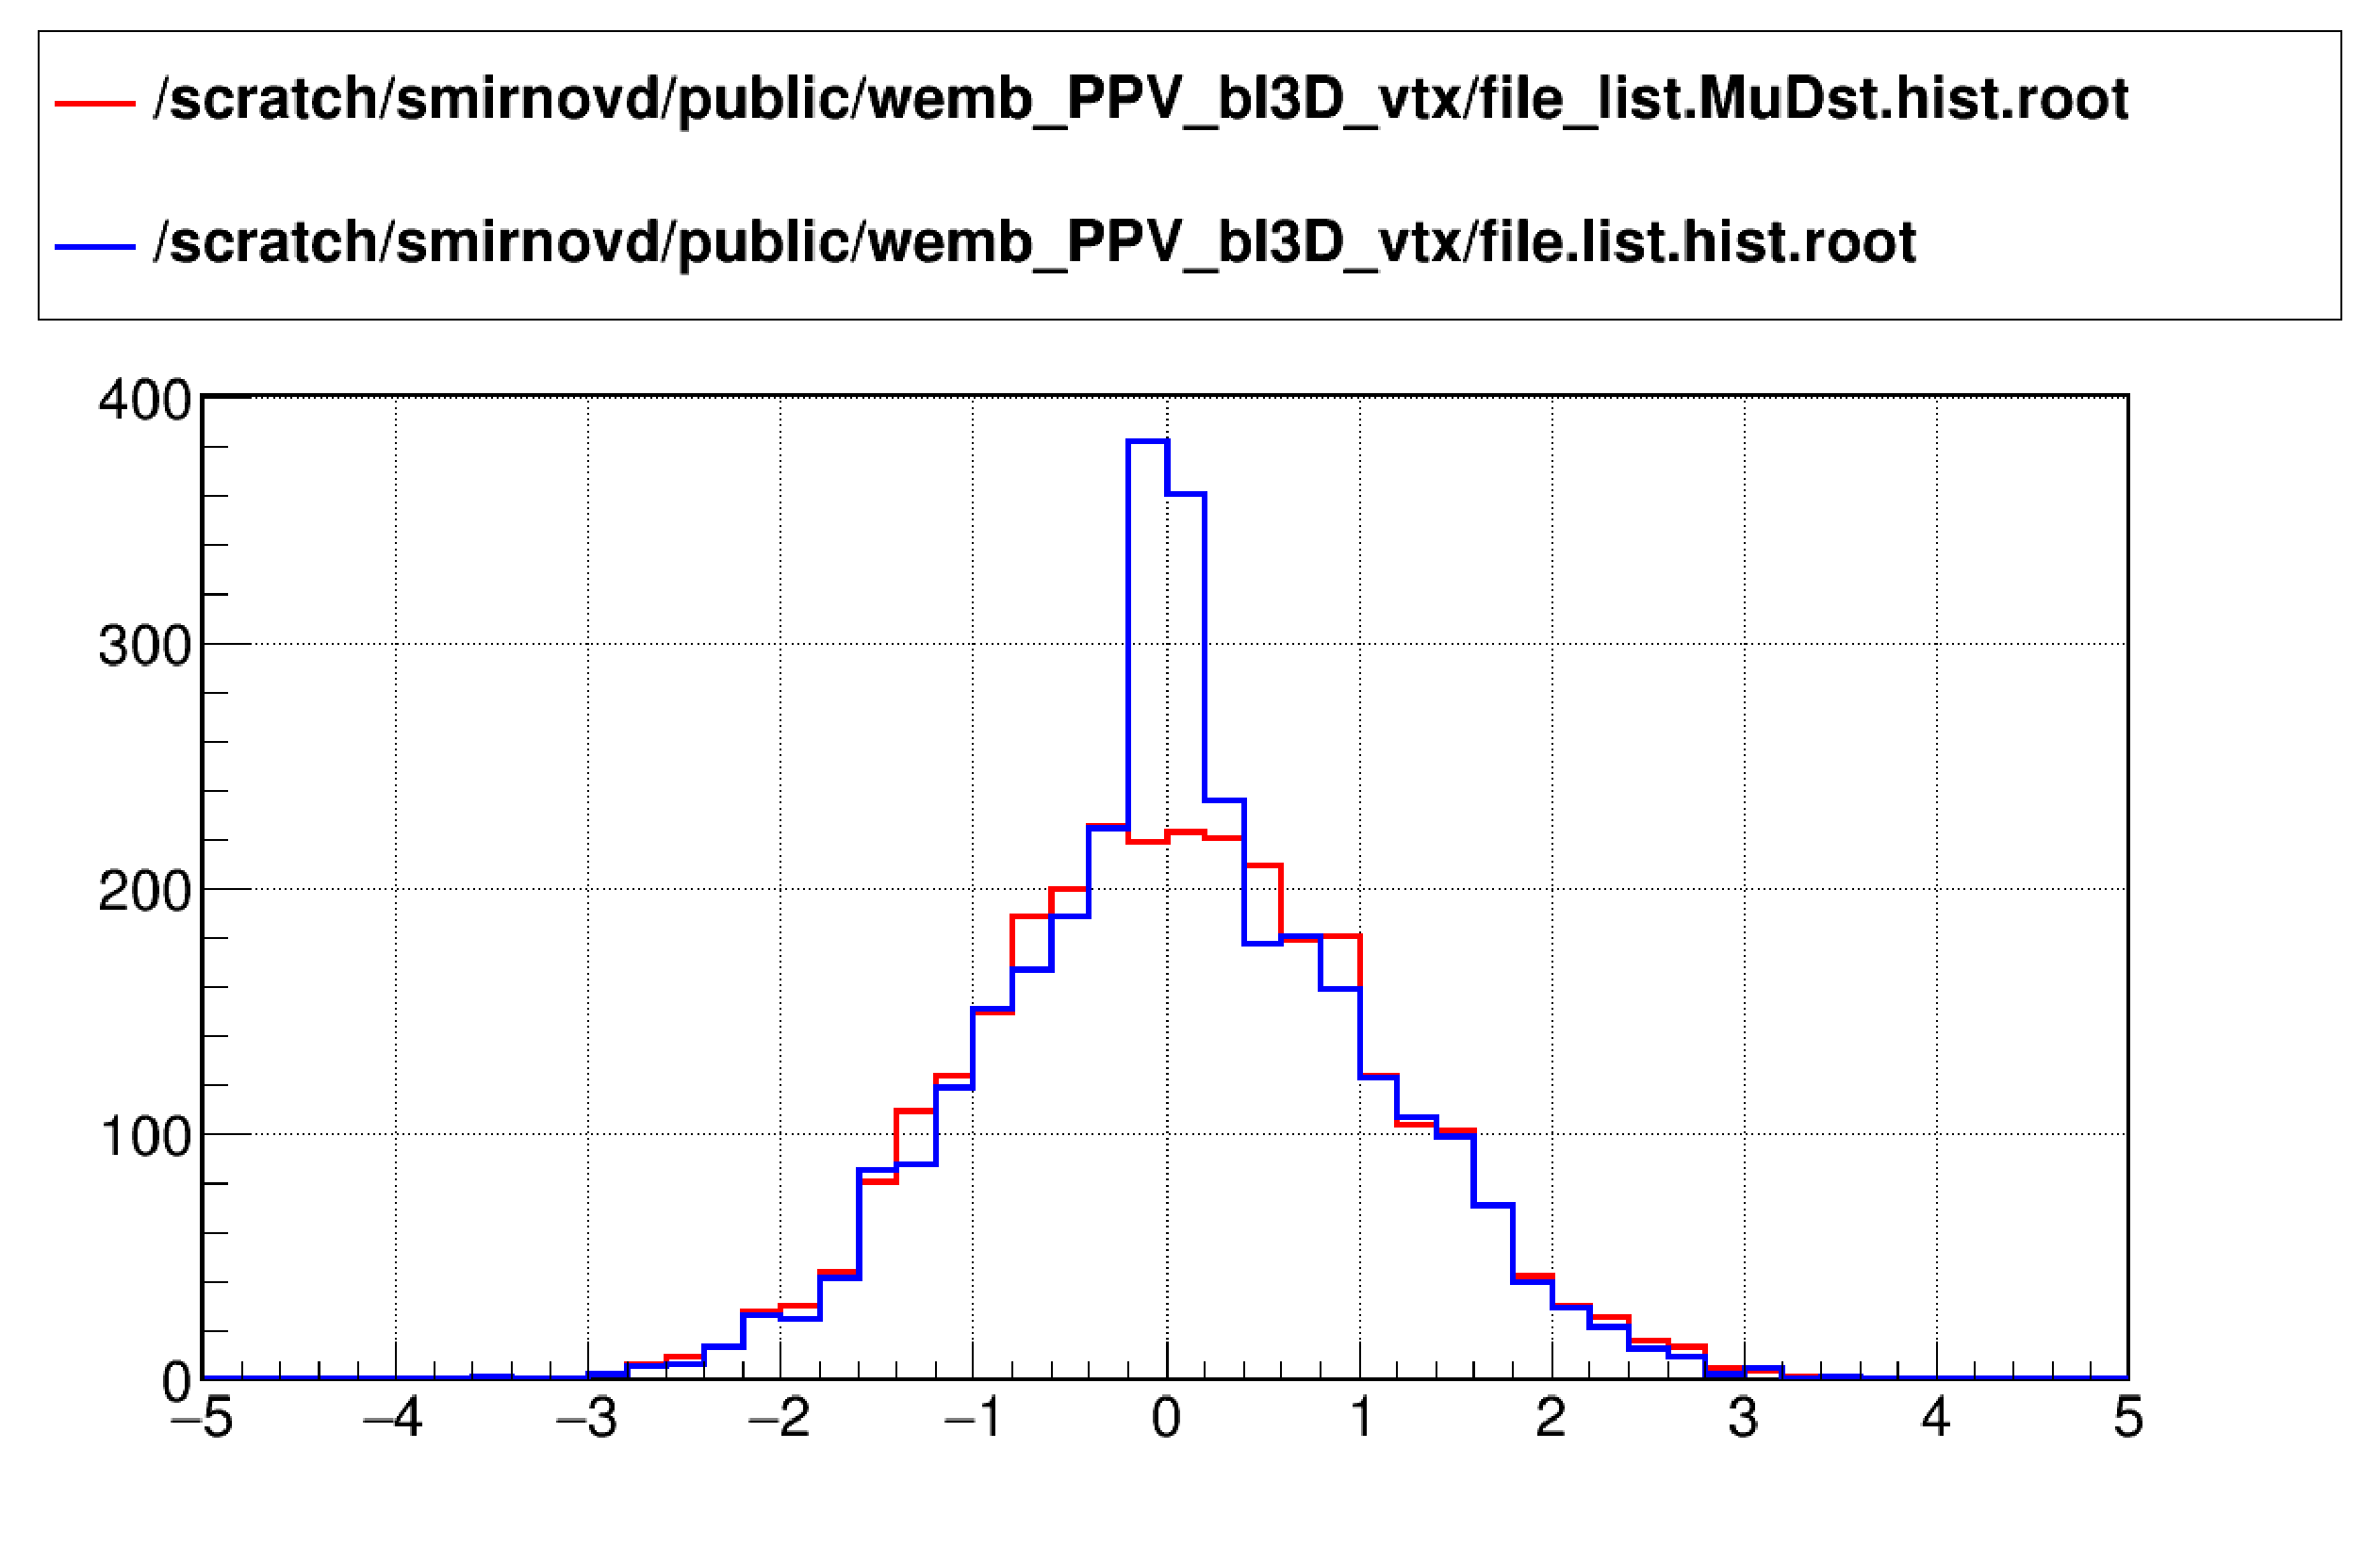
\includegraphics[height=0.5\textheight]{graphics/wemb_PPV_bl3D_muDst_vs_std_reco/vertex/hVertexPullY}}

\rput[t](0.5\textwidth,12){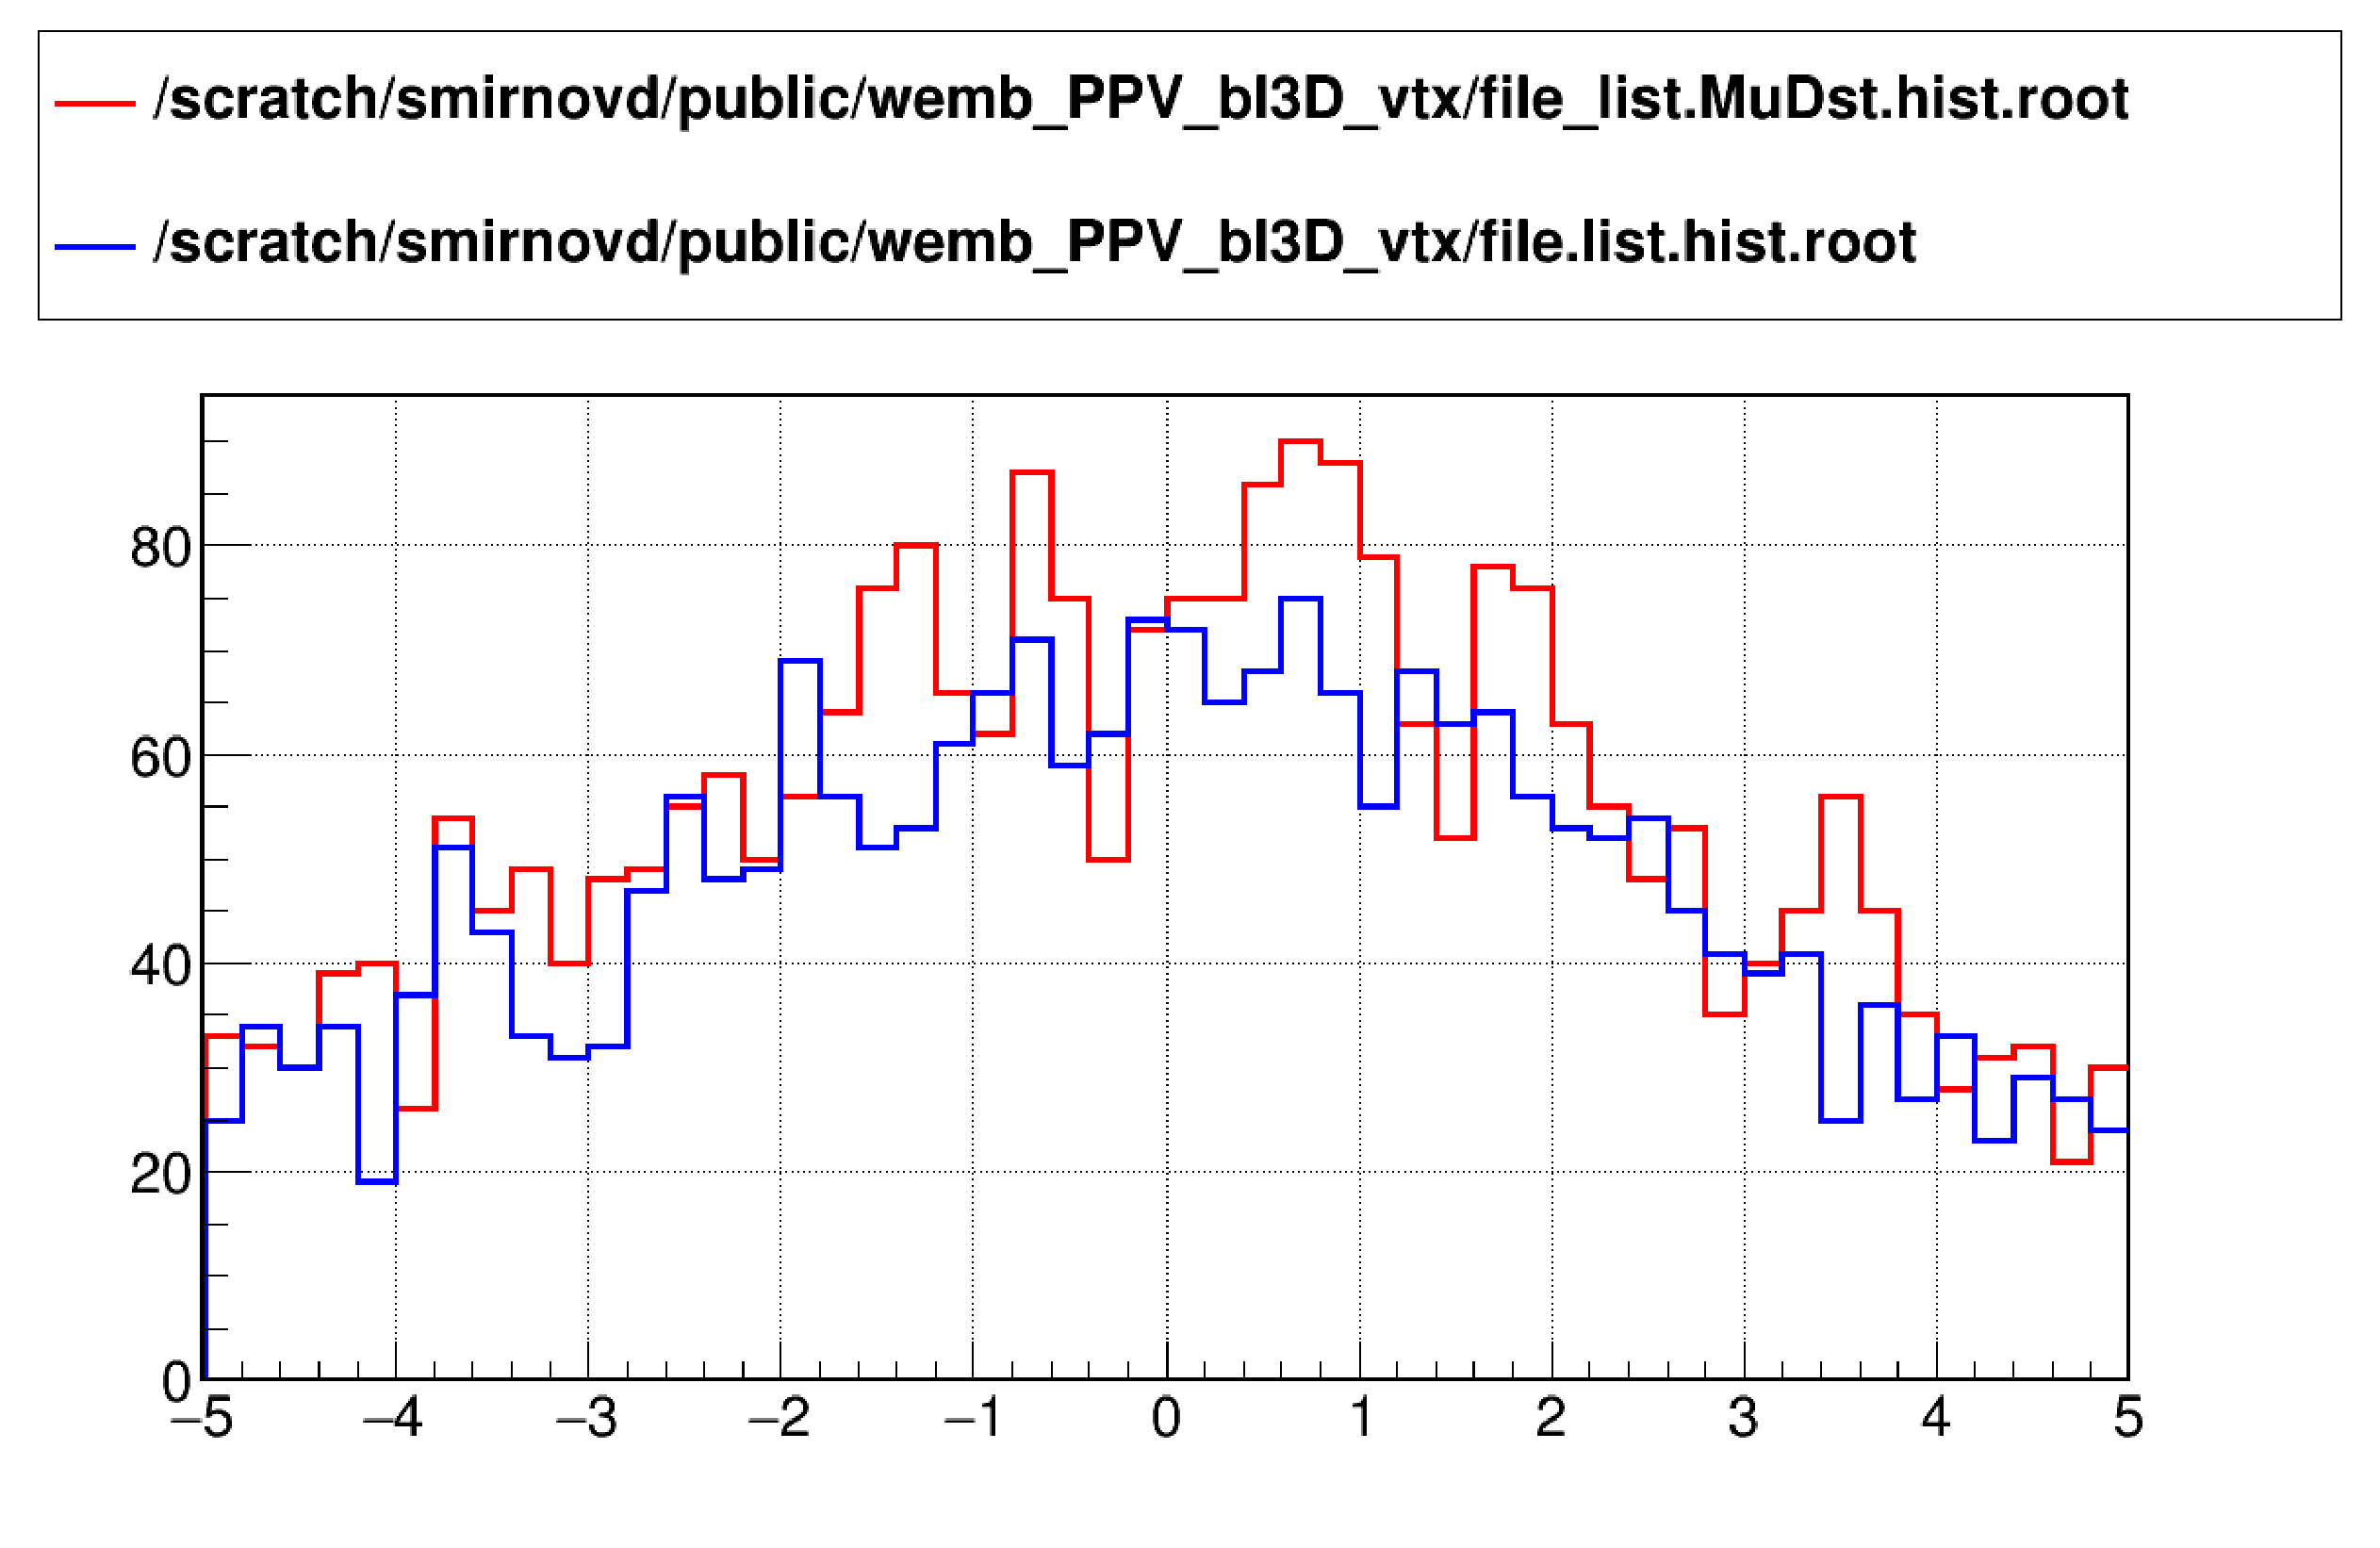
\includegraphics[height=0.5\textheight]{graphics/wemb_PPV_bl3D_muDst_vs_std_reco/vertex/hVertexPullZ}}


%\psgrid[gridlabels=0.7,subgriddiv=0, griddots=3](1,-1)(0,-3)(\textwidth,\textheight)

\end{pspicture}
%}}}



%===============================================================================
\myfoilhead{-30mm}{Summary}
%{{{

\noindent
\begin{pspicture}(0,0)(\textwidth,\textheight)



\rput(0.50\textwidth,0.45\textheight) {%
\begin{minipage}{0.90\textwidth}

\raggedright

\begin{list}{\labelitemi}{\setlength{\itemsep}{0mm}
                          \setlength{\topsep}{0mm}}

   \item Proof of concept: Vertices can be reconstructed using \StMuTrack-s

   \begin{list}{\labelitemii}{\setlength{\itemsep}{3mm}
                              \setlength{\topsep}{0mm}}

      \item Speed up factor for vertex studies $\sim 100$'s (no track (re-)reconstruction needed)

      \item Comparable vertex reconstruction efficiency as with \StTrack-s

   \end{list}

   \item Next steps

   \begin{list}{\labelitemii}{\setlength{\itemsep}{3mm}
                              \setlength{\topsep}{0mm}}

      \item Investigate systematic shifts in pull distributions (3D fit)

      \item Refit StMuTrack-s (i.e. innermost track state)

   \end{list}

\end{list}

\end{minipage}
}



%\psgrid[gridlabels=0.7,subgriddiv=0, griddots=3](1,-1)(0,-3)(\textwidth,\textheight)

\end{pspicture}
%}}}



%===============================================================================
\label{slide:last}

\end{document}
